\documentclass[a4paper,11pt]{article}

\usepackage[latin1]{inputenc}
\usepackage[T1]{fontenc}
\usepackage{bbm} %math chars
\usepackage{amsmath}
\usepackage{indentfirst}
\usepackage{fullpage} %minimizes the default margins
\usepackage{url}
\usepackage{graphicx}
\usepackage[center,footnotesize]{caption} %options des legendes des graphes
\usepackage[section]{placeins} %place les figures d'une section avant le debut de la suivante
\usepackage{subfig} %a) b) c)

\title{Exercises - Week 8}
\date{}
\author{Genomics and bioinformatics}

\begin{document}
\maketitle

\section{MSA with ClustalW}

\noindent Here is a summary of the main steps followed by ClustalW to generate the MSA. ClustalW first computes the optimal global alignment for every pair of sequences and then the distance score is set to be $1-y/x$, where $x$ and $y$ are the number of non-gap positions and the number of identical positions, respectively. The guide tree is then built according to the distance matrix (and not the raw alignment scores) using the neighbour joining algorithm presented in the lectures. The last step involves doing profile-profile alignments and may be computed using dynamic programming to with some PSP score. 

\begin{figure}[h!]
\hspace{-10mm}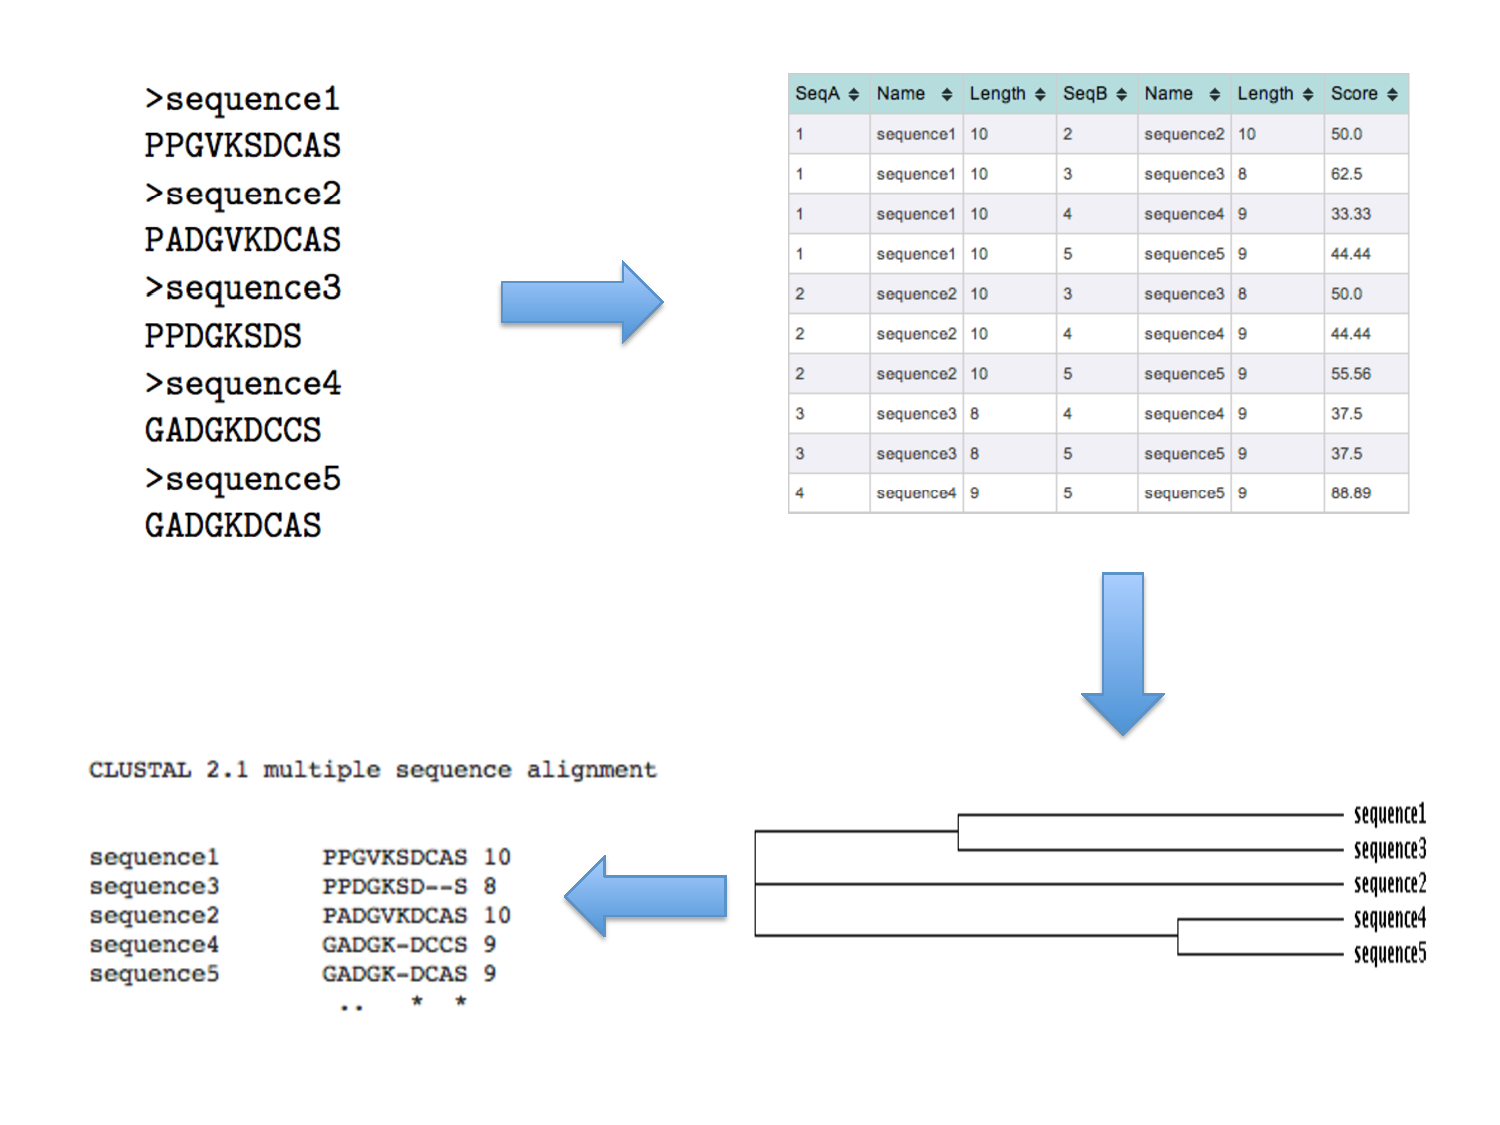
\includegraphics[width=17.5cm]{Fig1.pdf}
\end{figure}

\noindent Using the PAM250 scoring matrix with a gap penalty of -10, one can compute the SP score of the MSA by hands using the formula presented in the course. It is however more convenient to write a code (see \verb|MSA_SP_score.py|) to do this task. We find a SP score of 101.

\end{document}











